\documentclass[letterpaper,11pt,oneside,reqno]{amsart}
\usepackage[T2A]{fontenc}
\usepackage[utf8]{inputenc}
\usepackage[english]{babel}
\usepackage{amsmath,amssymb,amsthm,amsfonts,upgreek}
\usepackage{hyperref}
\usepackage{enumerate}
\usepackage{graphicx}
\usepackage[mathscr]{euscript}
\usepackage{color,tikz}
\usepackage[DIV15]{typearea}
% \usepackage[width=.75\textwidth]{caption}
\allowdisplaybreaks
\numberwithin{equation}{section}
\usepackage{listings}

\synctex=1
\newcommand{\note}[1]{\textsc{\color{blue}(#1)}}
\newcounter{lecture}
\newcommand{\lect}[1]{\bigskip\addtocounter{lecture}{1}\noindent{\Large\textbf{\color{red}Lecture \#\arabic{lecture} on #1 \hrulefill}}\bigskip}
\usepackage{refcheck}

%%%%%%%%%%%%%%%%%%%%%%%%%%%%%%%%%%%%%%%%%%%%%%%%%%%%%%%%%%%%
\newcommand{\SC}{\mathsf{SC}}
\DeclareMathOperator{\EE}{\mathbb{E}}
\DeclareMathOperator{\VAR}{\mathrm{Var}}
\DeclareMathOperator{\PP}{\mathbb{P}}

 
%%%%%%%%%%%%%%%%%%%%%%%%%%%%%%%%%%%%%%%%%%%%%%%%%%%%%%%%%%%%
\newtheorem{proposition}{Proposition}[section]
\newtheorem{lemma}[proposition]{Lemma}
\newtheorem{corollary}[proposition]{Corollary}
\newtheorem{theorem}[proposition]{Theorem}
\theoremstyle{definition}
\newtheorem{definition}[proposition]{Definition}
\newtheorem{remark}[proposition]{Remark}
\newtheorem{example}[proposition]{Example}
\newtheorem{exercise}[proposition]{Exercise}
%%%%%%%%%%%%%%%%%%%%%%%%%%%%%%%%%%%%%%%%%%%%%%%%%%%%%%%%%%%%

\begin{document}

\title[Notes on random matrices]{Notes on random matrices}

\author[L. Petrov]{Leonid Petrov}
\date{\today}
\maketitle

\begin{center}
	(notes by 
	Stephen Hardy;
	Bryce Terwilliger; \ldots)
\end{center}

\begin{abstract}
	These are notes for the MATH 8380 ``Random Matrices'' course at the
	University of Virginia in Spring 2016. The notes are constantly updated,
	and the latest version can be found at the \texttt{git} repository
	\url{https://github.com/lenis2000/RMT_Spring_2016}
\end{abstract}

\bigskip

\begin{center}
\noindent\note{before \TeX{}ing, please familiarize yourself with style suggestions at\\
\url{https://github.com/lenis2000/RMT_Spring_2016/blob/master/TeXing.md}}
\end{center}
\bigskip

\setcounter{tocdepth}{1}
\tableofcontents
\setcounter{tocdepth}{3}

\lect{1/20/2016}

\section{Introduction} % (fold)
\label{sec:introduction}

\subsection{Matrices and eigenvalues} % (fold)
\label{sub:object_of_study}

The study of random matrices as a field is a patchwork of many fields.  The
main object we study is a probability distribution on a certain subset of the
set of matrices $\mathrm{Mat}(N\times N,\mathbb R \text{ or } \mathbb C)$,
thus giving us a random matrix $A$.

\begin{definition}
An {\it eigenvalue} $\lambda$ of the matrix $A$ is a root of the polynomial
$f(\lambda)=\text{det}(A-\lambda I)$, where $I$ is the identity matrix 
(we use this notation throughout the notes).  
Equivalently, $\lambda$ is an
eigenvalue if $A$ if the matrix $A-\lambda I$ is not invertible. This second
way of defining eigenvalues in fact works even when $A$ is not a finite
size matrix, but an operator in some infinite-dimensional space.
\end{definition}

We will largely be only concerned with real eigenvalues.  That is the
eigenvalues of a real symmetric matrix over $\mathbb R$ or Hermitian over
$\mathbb C$ that is where $A^*=A$
(here and everywhere below
$A^*$ means $\overline{A^{T}}$, i.e., transposition and complex conjugation).

\begin{remark}\label{rmk:complex_eigenvalues}
	The case when eigenvalues can be complex is also studied in
	the theory of random matrices, sometimes under the keyword \emph{complex
	random matrices}. 
	This area is more modern and is actively developing now.
	See, for example, \cite{gotze2010circular} for a discussion of the law of 
	large numbers.
\end{remark}

\begin{proposition}
Every eigenvalue of a Hermitian matrix is real.
\end{proposition}
\begin{proof}
Let $A$ be a Hermitian matrix, so that $A^*=A$.
Let $\lambda$ be an eigenvalue of $A$.  Let $v$ be a non-zero vector in the null
space of $A-\lambda I$.  Let $a=\overline{ v^{T}}v=|v|^2$, so
that $a$ is a positive real number.  Let $b=\overline{ v^{T}}A
v$.  Then $\bar b=\overline{ b^{T}}=\overline{\overline{
v^{T}}Av}^{T}=\overline{
v^{T}}\bar A^{T} v=\overline{
v^{T}}Av=b$, so $b$ is real.  Since $b=\lambda a$, $\lambda$
must be real. 
\end{proof}

Let $\mathcal H_N$ be the set of $N\times N$ Hermitian matrices.  For each
$N$, let $\mu_N$ be a probability measure on $\mathcal H_N$ (it can be
supported not by  the whole $\mathcal H_N$, but by a subset of it, too).  Then
for each matrix $A\in \mathcal H_N$ we may order the real eigenvalues
$\lambda_1\geq \cdots \geq \lambda_N$ of $A$ (the collection of eigenvalues
is called the \emph{spectrum} of $A$).

A collection of probability measures $\mu_N$ on $\mathcal H_N$ for each
$N\ge1$ is said to be a \emph{random matrix ensemble}. For such an ensemble,
the eigenvalues $\lambda_1^{(N)}\geq \cdots \geq \lambda_N^{(N)}$ of matrices
$N$ form random point configurations on $\mathbb{R}$ with growing numbers of points.
Our main goal is to study the asymptotic properties of these collections of points on $\mathbb{R}$,
as $N\to\infty$.

% subsection object_of_study (end)

\subsection{Why study random matrices?} % (fold)
\label{sub:why_study_random_matrices_}

Let us briefly discuss five possible motivations to study random matrices and asymptotic distributions of 
random matrix spectra.

\subsubsection{}

Matrices are a natural generalization of real numbers, so studying them would
seem natural from a  pure probability point of view. However, the development
of the theory of Random Matrices was much application driven.

\subsubsection{Hurwitz and theory of invariants} 

A. Hurwitz in the 1890s \cite{Hurwitz1897} computed the volume of orthogonal
and unitary groups of matrices.\footnote{The group $O(N)$
of orthogonal $N\times N$ matrices consists of matrices $O$ with real entries, 
for which $O^{T}O=OO^{T}=I$.
The group $U(N)$ of unitary 
$N\times N$ matrices consists of matrices $U$ with complex entries, 
for which $UU^{T}=U^{T}U=I$.
Both groups are \emph{compact}, and so possess finite Haar measures,
i.e., measures $\mu$ which are invariant under left and right shifts on the group.} 
For example, $U(1)$, the set of unitary
$1\times 1$ unitary matrices --- the unit circle --- has volume $2\pi$.  For general $N$, the
volume of $U(N)$ is the normalization constant $Z_N=\int_{U(N)} 1\cdot d(\mathrm{Haar}_N)$ in probabilistic integrals
over the Haar measure on the unitary group,
\begin{align*}
  	Z_N=2^{N(N+1)/2}\prod_{k=1}^{N}\frac{\pi^{k}}{\Gamma(k)}=2^{N(N+1)/2}\prod_{k=1}^{N}\frac{\pi^{k}}{(k-1)!}.
\end{align*}
See
\cite{diaconis2015hurwitz} for a recent survey.

\subsubsection{Statistics} 

J. Wishart in 1928 \cite{wishart1928generalised} considered random covariance matrices of 
vector-valued data. For testing the hypothesis of independence of components of the vector,
it is natural to study the distribution of the random covariance matrix 
of the uncorrelated vector (the null-hypothesis distribution). Let us assume that the components
of the vector are identically distributed.

This latter matrix ensemble (called the \emph{Wishart ensemble})
can be constructed by taking a rectangular matrix $Y$ with independent (or uncorrelated) 
identically distributed entries, and taking $A=Y^{T}Y$. Then $A$ is a square matrix
which is said to have the (\emph{real}) \emph{Wishart distribution}. 

For the purposes of statistics, the distribution of the Wishart matrix $A$ should be 
compared with the distribution under the alternate hypothesis that the entries of the vector are correlated.
For certain assumed nature of the correlation structure, this leads to
considering \emph{spiked random matrices} of the form $A+R$, where $A$
is Wishart and $R$ is a finite-rank perturbation. It turns out that sometimes the 
presence of a nonzero matrix $R$ may be detected by looking at the spectrum of $A+R$,
which again leads to considering spectra of random matrices.
One reference (among many others which are not mentioned) 
relevant for the current research on spiked random matrices is
\cite{BBR2005phase}.

\subsubsection{Nuclear physics} 

Active development of the theory of random matrices begins in the 1950s when
Wigner, Dyson, Mehta, and their collaborators explored nuclear physics
applications.  In nuclear quantum physics a state of a system is an operator
on an $L^2$ space of functions; its eigenvalues are the energy levels of the
system.  For  large nuclei it is difficult to analyze the operator in $L^2$
directly, but Wigner postulated that differences in energy levels could be
modeled by differences in eigenvalues of certain classes of matrices under
appropriate probability measures. That is, the collections $\{\Delta E_i\}$
and $\{\lambda_i-\lambda_{i+1}\}$ should be statistically close. Moreover, the
random matrix ensemble should have the same symmetry as that quantum system.
The symmetry classes of random matrices are discussed in detail in a recent
survey \cite{Zirnbauer2010}. Dyson proposed a model of stochastic dynamics of
energies (eigenvalues of random matrices). We will study the Dyson's Brownian
motion later. 

Section 1.1 of the book \cite{mehta2004random} contains a nice outline of 
physical applications of random matrices.

\subsubsection{Number theory} 

Dyson and Montgomery uncovered number theoretic applications of random matrices 
in the 1970's \cite{montgomery1973pair}, with Odlyzko in the 1980's \cite{odlyzko1987distribution} providing powerful numerical simulations.

Consider the Riemann Zeta Function
\begin{equation*}
\zeta(s)=\sum_{n=1}^{\infty}\frac{1}{n^s} \qquad \text{ for } s\in \mathbb C \text{ with the real part of } s>1
\end{equation*}

Riemann showed that $\zeta(s)$ can be analytically continued to a function on
$\mathbb C$ with a pole at $s=1$.  The famous Riemann hypothesis is that all
the zeroes of the Zeta function with real part greater than 0 lie on the
\emph{critical line} $\frac{1}2+i t$.  It turns out that the distribution of
the zeroes on the critical line can be linked to the distribution of
eigenvalues of random matrices.  Consider the zeros $\frac12+it_n$ of the zeta function
with $t_n\in\mathbb{R}$. Let us define
\begin{equation*}
w_n=\frac{t_n}{2\pi}\log\left(\frac{|t_n|}{2\pi}\right),
\end{equation*}
then $\displaystyle \lim_{L\to\infty} \frac{1}{L} \#\left\{w_n\in [0,L]\right\}=1$, i.e., the 
average density of the $w_n$'s is $1$.
The theorem/conjecture of Montgomery\footnote{Depending in part
on the Riemann hypothesis and in part on 
how strong is the assumed convergence in \eqref{Montgomery_zeta}.} states that the pair correlations of the 
zeroes of the zeta function have the form
\begin{equation}\label{Montgomery_zeta}
	\lim_{L\to\infty} \frac{1}{L}\# \left\{\begin{array}{c} w_n\in [0,L] \\ \alpha\leq w_n-w_m\leq \beta \end{array}\right\} 
	\sim \int_\alpha^\beta \left(\delta(x)+1 -\frac{\sin^2(\pi x)}{\pi^2 x^2}\right)\, dx,
\end{equation}
where $\delta(x)$ is the Dirac delta.
Further details on this and other connections
between number theory and random matrices
can be found in \cite{keating2000random}, \cite{keating2006random}.

\begin{remark}
	There are accounts of Montgomery 
	meeting Dyson at teatime at the IAS; the latter pointed
	out the connection between Montgomery's formula and the eigenvalue
	distributions of random matrices. 
	A quick Internet search lead to the following links containing details:
	\url{https://www.ias.edu/articles/hugh-montgomery} and
	\url{http://empslocal.ex.ac.uk/people/staff/mrwatkin//zeta/dyson.htm}.
\end{remark}


% subsection why_study_random_matrices_ (end)

\subsection{Course outline} % (fold)
\label{sub:goals_for_the_course}

The course will consist of five main parts, with the last part being optional:

\begin{enumerate}[\bf1.]
	\item Limit shape results for random matrices (such as Wigner's Semicircle Law). Connections to Free Probability.
	\item Concrete ensembles of random matrices (GUE, circular, and Beta ensembles). Bulk and edge asymptotics via exact computations. Connection to determinantal point processes.
	\item Dyson's Brownian Motion and related stochastic calculus.
	\item Universality of random matrix asymptotics.
	\item (optional, depending on time available) Discrete analogues of random matrix models: random permutations, random tilings, interacting particle systems.
\end{enumerate}

% subsection goals_for_the_course (end)

% section introduction (end)

\section{Wigner's Semicircle Law and its combinatorial proof} % (fold)
\label{sec:wigner_s_semicircle_law}

After discussing the object and motivations for studying random matrices, let
us proceed to the first part of the course --- the laws of large numbers
for the eigenvalue distributions of random matrices. 
The first of these laws of large numbers is the 
\emph{Wigner's Semicircle Law}. It dates back to 
\cite{wigner1955characteristic}.

\subsection{Real Wigner matrices} % (fold)
\label{sub:real_wigner_matrices}

A particular ensemble of random matrices is the \emph{real Wigner matrices}.
Let $A\in \mathrm{Mat}(N\times N,\mathbb R)$ with $A=(a_{ij})_{i,j=1}^N$ such
that $a_{ij}=a_{ji}$. To describe the distribution of the random matrix $A$ we only need to
describe the upper triangular portion of $A$.

\begin{definition}\label{def:real_Wigner}
The law of the real Wigner $N\times N$ matrix is described as follows:
\begin{itemize}
	\item $\{a_{ij}\}_{i\leq j}$ is an independent collection of random variables
	\item $\{a_{ii}\}_{i=1}^N$ is iid\footnote{Independent identically
	distributed.}, and $\{a_{ij}\}_{i<j}$ is iid.
	\item $\EE a_{ij}=0$ for all $i,j$; $\EE a_{ij}^2=2$ for $i=j$; and $\EE a_{ij}^2=1$ for $i\neq j$.
	\item all moments of $a_{ij}$ are finite.
\end{itemize}
The last condition greatly simplifies technicalities of the proofs,
but most results on real Wigner matrices hold under weaker assumptions.
\end{definition}

\begin{example}
A large class of Wigner random matrices
(which helps justify why in $A$ the variances on the diagonal must be twice the 
off-diagonal
variances) can be constructed as follows.
Suppose the collection of random variables $x_{ij}$ for $1\leq i,j\leq N$ is iid with $\EE x_{ij}=0$ and $\EE x_{ij}^2=1$.  Let $X=(x_{ij})$ be an $N\times N$ matrix.  Define
\begin{equation*}
	A:=\frac{X+X^T}{\sqrt{2}}.
\end{equation*}
One readily sees that $A$ is real Wigner. Namely, for example,
$a_{11}=\frac{x_{11}+x_{11}}{\sqrt 2}=\sqrt 2 x_{11}$, so $\EE a_{11}=0$ 
and $\EE a_{11}^2=2\EE x_{11}^2=2$.  If $N\geq 2$ then $a_{12}=a_{21}$ with $a_{12}=\frac{x_{12}+x_{21}}{\sqrt 2}$, 
and we have $\EE a_{12}=0$ and $\VAR a_{12}=\frac{1}{2}\VAR(x_{12}+x_{21})=1$ because $x_{12}$ and $x_{21}$ are independent.
\end{example}

% subsection real_wigner_matrices (end)

\subsection{Gaussian Orthogonal Ensemble} % (fold)
\label{sub:gaussian_orthogonal_ensemble}

A special case of real Wigner matrices  is when each $a_{ij}$ is Gaussian.
This case is called the \emph{Gaussian Orthogonal Ensemble} (\emph{GOE}).

\begin{lemma}
	The distribution of the GOE is orthogonally invariant, that is,
	if $A$ has the GOE distribution and $O\in O(N)$ is a fixed
	orthogonal matrix, then $OAO^{T}$ has the same probability distribution~as~$A$.
\end{lemma}
\begin{proof}
	It is not hard to check that the
	probability density of $A$ with respect to the 
	Lebesgue measure on $\mathrm{Mat}(N\times N,\mathbb R)$
	(this space is isomorphic to $\mathbb{R}^{N(N+1)/2}$
	by considering the upper triangular part)
	has the form
	\begin{align*}
		f(A)=c \exp(-\mathop{\mathrm{tr}}(A^2)),
	\end{align*}
	where $c$ is a normalization constant.\footnote{Here 
	and below $\mathop{\mathrm{tr}}(A)=a_{11}+a_{22}+\ldots+a_{NN}$ 
	is the trace of a matrix.}  Since the matrix trace
	is invariant under cyclical permutations, 
	\begin{align*}
		\mathop{\mathrm{tr}}(OA^2O^{T})
		=\mathop{\mathrm{tr}}(A^2O^{T}O)
		=\mathop{\mathrm{tr}}(A^2).
	\end{align*}
	Thus, $OA^2O^{T}\stackrel{\mathcal D}{=} A$.
\end{proof}

We will discuss the GOE (and its close relative GUE, Gaussian Unitary Ensemble)
in detail in the course later, but for now we will focus on 
properties of real Wigner matrices with general entry distribution.

% subsection gaussian_orthogonal_ensemble (end)

\subsection{Formulation of the Wigner Semicircle Law} % (fold)
\label{sub:formulation_of_the_wigner_semicircle_law}

For a real Wigner matrix $A_N\in\mathrm{Mat}(N\times N)$ let
$\lambda_1^{(N)}\geq \cdots \geq \lambda_N^{(N)}$ be the eigenvalues of $A_N$.
The \emph{empirical distribution of the eigenvalues} is
\begin{equation}\label{EmpiricalDistributionOfEigenvalues}
	L_N=\frac{1}{N}\sum_{i=1}^N \delta_{N^{-1/2}\lambda_{i}^{(N)}}.
\end{equation}
That is, we put delta masses of size $1/N$ into the
$N$ positions of rescaled eigenvalues 
$\lambda_{i}^{(N)}/\sqrt N$. This rescaling will turn out to be appropriate for the 
law of large numbers.
Note that $L_N$ is a probability measure on $\mathbb{R}$.

\begin{remark}
	For the purposes of asymptotic statements, we will always assume that the 
	off-diagonal entries of real Wigner matrices 
	$A=A_N$ have the same fixed distribution independent of $N$,
	and similarly the diagonal entries 
	have the same fixed (but different) distribution.
\end{remark}

\begin{figure}[htbp]
	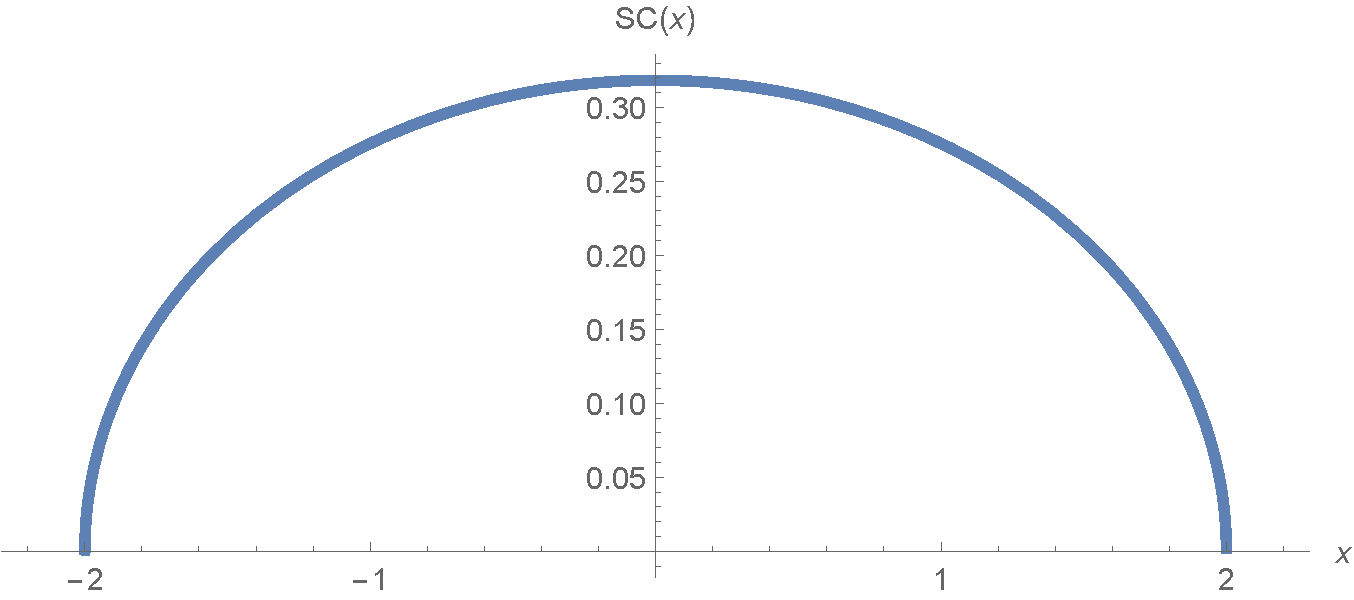
\includegraphics[width=.5\textwidth]{img/SC.pdf}
	\caption{Semicircle density $\SC(x)$.}
	\label{fig:semicircle}
\end{figure}

\begin{figure}[htbp]
	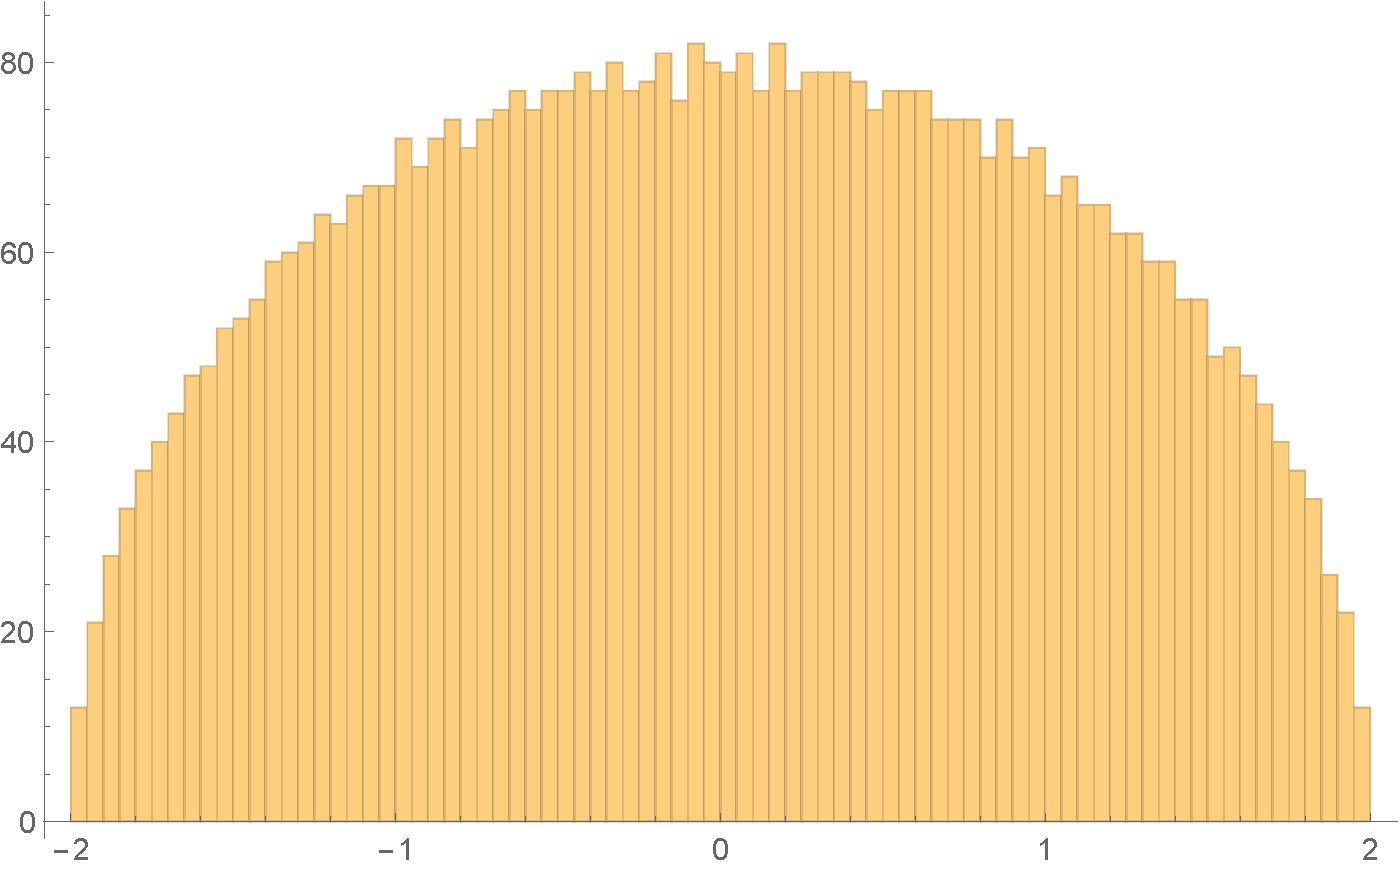
\includegraphics[width=.5\textwidth]{img/Wigner1.pdf}
	\caption{Histogram of the empirical distribution 
	$L_N$ for $N=5000$.}
	\label{fig:Wigner}
\end{figure}

\begin{definition}
	The semicircle distribution $\SC$ is 
	a fixed probability distribution on $\mathbb{R}$
	supported on $[-2,2]$
	which is absolutely continuous with respect to the
	Lebesgue measure and has the density
	\begin{equation}\label{SemicircleDistribution}
		\SC(x):=\frac{1}{2\pi}\sqrt{4-x^2}, \qquad -2\leq x\leq 2.
	\end{equation}
	See Fig.~\ref{fig:semicircle}.

	Note that slightly abusing the notation, by $\SC$ we will denote both the
	semicircle distribution and its probability density \eqref{SemicircleDistribution}.
\end{definition}

\begin{theorem}[Wigner's Semicircle Law]\label{thm:SemicircleLaw}
	As $N\to\infty$,
	the empirical distributions 
	$L_N$ converge weakly, in probability to the 
	semicircle distribution $\SC$.
\end{theorem}

Let us explain what we mean by convergence ``weakly in probability''. Formally this means that
for any bounded continuous function $f$ on $\mathbb R$ ($f\in C_B(\mathbb R)$) and each $\epsilon>0$ we have 
\begin{equation}\label{WignerSemicircleLaw}
\lim_{N\to\infty}\mathbb P\left(\left|\int_{\mathbb R} f\,dL_N-\int_{\mathbb R} f\,d\SC\right|>\epsilon\right)=0.
\end{equation}
That is, ``in probability'' means the usual convergence in probability  of
random elements $L_N$ to a (nonrandom) element $\SC$.  On the other hand,
``weakly'' specifies the metric on the space of probability measures on
$\mathbb{R}$ (to which all $L_N$ and $\SC$ belong). Convergence of probability
measures in this metric simply means weak convergence of probability measures
on $\mathbb{R}$.

In other words,
let us use a convenient notation for the pairing $\langle f,\mu\rangle
=\int_{\mathbb R} f\,d\mu=\int_{\mathbb R}f(x)\,\mu(dx)$ for a given
function $f$ and measure $\mu$.  If $\mu$ is a random measure (such as $L_N$,
since $L_N$ depends on $A_N$ which is random), then $\langle f,\mu\rangle$ is
a random element of $\mathbb R$ (usually we say random variable).  Since $\SC$
is not random, the pairing $\langle f,\SC\rangle$ is a fixed number for a given function $f$.  The
Semicircle Law thus states that for any given $f\in C_B(\mathbb R)$ the random variable
$\langle f,L_N\rangle$ converges in probability to the constant $\langle f,\SC\rangle$ which may be written as
\begin{equation}\label{WignerSemicircleLaw_langle}
\forall \epsilon>0,\qquad \lim_{N\to\infty}\PP\left(\left|\langle f,L_N\rangle-\langle f,\SC\rangle\right|>\epsilon\right)=0,
\end{equation}
which is the same as \eqref{WignerSemicircleLaw}.

\begin{remark}
	This type of convergence is reminiscent of the classical weak law of large numbers: for
	$\{X_i\}_{i=1}^\infty$ iid random variables with $\EE|X_1| <\infty$, the random
	variables $\dfrac{1}N\sum_{i=1}^N X_i$ converge to the constant $\EE X_1$ in probability as $N\to\infty$.
\end{remark}

% subsection formulation_of_the_wigner_semicircle_law (end)

\lect{1/25/2016}

\subsection{Strategy of the proof} % (fold)
\label{sub:strategy_of_the_proof}

We will employ the following strategy in our proof of the Wigner's semicircle
law. This is only the first of the proofs we will consider, and it is based on
the computation of moments and on the related combinatorics. Recall that for a
probability measure $\mu$ the quantities $\langle x^{k},\mu\rangle$,
$k=0,1,2,\ldots$, are called the \emph{moments} of $\mu$.

First, in \S \ref{sub:moments_of_the_semicircle_distribution}
we will compute the moments  $m_k:=\langle x^k, \SC\rangle$ of the
limiting semicircle distribution, and identify the answer in terms of the
Catalan numbers. Our second step in the proof is to show the convergence
$\lim_{N\to\infty}\EE \langle x^k,L_N\rangle = m_k$ for each $k$. We do this in \S \ref{sub:convergence_of_expectations_}
below.
The third
step (in \S \ref{sub:variances_langle_x_k_l_nrangleto0_}) 
is to show that  the variance of $\langle x^k,L_N\rangle$ goes to zero as
$N\to\infty$ for each $k$. Finally, to complete the proof we will need to
justify that  the convergence \eqref{WignerSemicircleLaw_langle} for any
function $f(x)$ follows from the case of $f(x)=x^{k}$, $k=0,1,2,\ldots$.
This is done in \S \ref{sub:completing_the_proof_WSCL}.

% subsection strategy_of_the_proof (end)

\subsection{Moments of the semicircle distribution} % (fold)
\label{sub:moments_of_the_semicircle_distribution}

Here we will compute the moments of the semicircle distribution:
\begin{equation*}
m_k=\langle x^k, \SC\rangle
=\int_{-2}^2 x^k\, \SC(x)\,dx
=\int_{-2}^2 x^k \left( \frac{\sqrt{4-x^2}}{2\pi}\right)\,dx.
\end{equation*}

Clearly, by symmetry we have $m_k=0$ for $k$ odd. If $k$ is even, let us perform a trigonometric substitution
$x=2\sin \theta$, $-\frac\pi2\le \theta\le \frac\pi2$, in the above integral:
\begin{align}\label{SC_moments_m_2k}
	m_{2k}=\frac{2^{2k+1}}{\pi}\int_{-\frac\pi2}^{\frac\pi2}\sin^{2k}\theta\cos^{2}\theta \,d\theta.
\end{align}

\begin{lemma}
	We have
	\begin{align*}
		\frac{1}{\pi}\int_{-\frac\pi2}^{\frac\pi2}\sin^{2k}\theta\, d\theta=
		\frac{(2k-1)!!}{2^k k!},
	\end{align*}
	where recall that $(2k-1)!!=1\cdot 3\cdot 5\cdots (2k-3)(2k-1)$.
\end{lemma}	
\begin{proof}
	Denote the integral in the right-hand side by $\alpha_{k}$. Observe that $\alpha_0=1$.
	Integrating by parts for $k\ge1$, we have
	\begin{align*}
		\alpha_k=
		-\frac{1}{\pi}\int_{-\frac\pi2}^{\frac\pi2}\sin^{2k-1}\theta\, d(\cos\theta)
		=\frac{1}{\pi}\int_{-\frac\pi2}^{\frac\pi2}
		(2k-1)\sin^{2k-2}\theta\cos^{2}\theta\, d\theta
		=(2k-1)\alpha_{k-1}-(2k-1)\alpha_{k}.
	\end{align*}
	Therefore, the quantities $\alpha_k$ satisfy
	\begin{align*}
		\frac{\alpha_k}{\alpha_{k-1}}=\frac{2k-1}{2k},
	\end{align*}
	which is the same relation as for the quantities 
	$\frac{(2k-1)!!}{2^k k!}$.
	This completes the proof.		
\end{proof}
By relating $m_{2k}$ \eqref{SC_moments_m_2k} and $\alpha_k$ in the above lemma,
we see that the even moments of the semicircle distribution are given by 
\begin{align}\label{m_2k_Catalan}
	m_{2k}=\frac{1}{k+1}\binom{2k}{k},\qquad k=0,1,2,\ldots.
\end{align}
These quantities are called the \emph{Catalan numbers}.

% subsection moments_of_the_semicircle_distribution (end)

\subsection{Catalan numbers} % (fold)
\label{sub:catalan_numbers}

The Catalan numbers $C_k$ are defined as
\begin{align}\label{Catalan_def}
	C_k:=\frac{1}{k+1}\binom{2k}{k},\qquad
	k=0,1,2,\ldots.
\end{align}
The first twenty one of them are
\begin{align*}
	1,1,2,5,14,42,132,429,1430,4862,16796,58786,208012,742900,2674440,\\9694845,35357670,129644790,477638700,1767263190,6564120420.
\end{align*}
They are ubiquitous in combinatorics: for
example, there are more than 200 families of objects  enumerated by the
Catalan numbers \cite{stanley2015catalan}. A list of references and
properties of Catalan numbers may be found at \cite{CatalanOEIS}.

Here we will list a number of properties of the Catalan numbers which will be important 
for our proof of the semicircle law.

\subsubsection{Dyck paths} % (fold)
\label{ssub:dyck_paths}

\begin{definition}
	A \emph{Dyck path} of length $2n$ is a 
	sequence $d_0,d_1,\ldots,d_{2n}$ such that
	$d_0=d_{2n}=0$, $d_{i+1}-d_{i}=\pm1$ for all $i$,
	and that $d_i\ge0$ for all $i$. Graphically Dyck paths can be represented as 
	on Fig.~\ref{fig:Dyck}.
\end{definition}

\begin{figure}[htbp]
	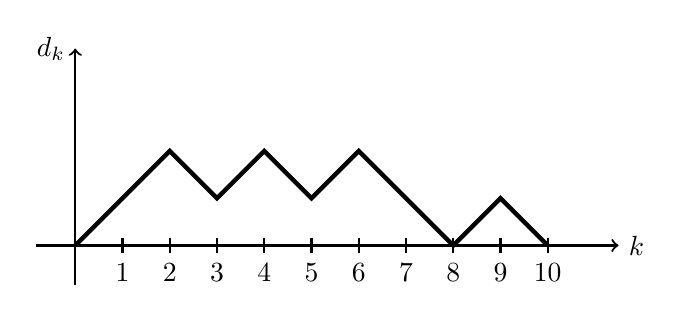
\begin{tikzpicture}[scale=1,thick]
		\draw[->] (-.5,0)--++(7.4,0) node [right] {$k$};
		\draw[->] (0,-.5)--++(0,3) node [left] {$d_k$};
		\foreach \ii in {1,...,10}
		{
			\draw (\ii*.6,.1)--++(0,-.2) node [below] {$\ii$};
		}
		\draw[ultra thick] (0,0)--++(.6,.6)--++(.6,.6)
		--++(.6,-.6)--++(.6,.6)--++(.6,-.6)
		--++(.6,.6)--++(.6,-.6)--++(.6,-.6)--++(.6,.6)--++(.6,-.6);
	\end{tikzpicture}
	\caption{A Dyck path of length $2n=10$.}
	\label{fig:Dyck}
\end{figure}

\begin{figure}[htbp]
	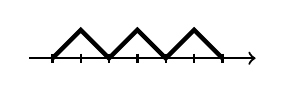
\begin{tikzpicture}[scale=.6,thick]
		\draw[->] (-.5,0)--++(4.8,0);
		\foreach \ii in {0,...,6}
		{
			\draw (\ii*.6,.1)--++(0,-.2);
		}
		\draw[ultra thick] 
		(0,0)--++(.6,.6)--++(.6,-.6)
		--++(.6,.6)--++(.6,-.6)--++(.6,.6)
		--++(.6,-.6);
	\end{tikzpicture}
	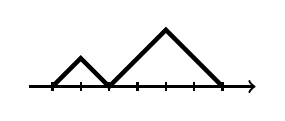
\begin{tikzpicture}[scale=.6,thick]
		\draw[->] (-.5,0)--++(4.8,0);
		\foreach \ii in {0,...,6}
		{
			\draw (\ii*.6,.1)--++(0,-.2);
		}
		\draw[ultra thick] 
		(0,0)--++(.6,.6)--++(.6,-.6)
		--++(.6,.6)--++(.6,.6)--++(.6,-.6)
		--++(.6,-.6);
	\end{tikzpicture}
	
	\rule{0pt}{34pt}
	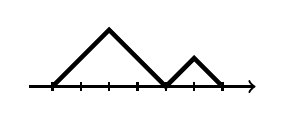
\begin{tikzpicture}[scale=.6,thick]
		\draw[->] (-.5,0)--++(4.8,0);
		\foreach \ii in {0,...,6}
		{
			\draw (\ii*.6,.1)--++(0,-.2);
		}
		\draw[ultra thick] 
		(0,0)--++(.6,.6)--++(.6,.6)
		--++(.6,-.6)--++(.6,-.6)--++(.6,.6)
		--++(.6,-.6);
	\end{tikzpicture}

	\rule{0pt}{41pt}
	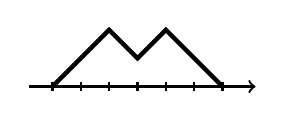
\begin{tikzpicture}[scale=.6,thick]
		\draw[->] (-.5,0)--++(4.8,0);
		\foreach \ii in {0,...,6}
		{
			\draw (\ii*.6,.1)--++(0,-.2);
		}
		\draw[ultra thick] 
		(0,0)--++(.6,.6)--++(.6,.6)
		--++(.6,-.6)--++(.6,.6)--++(.6,-.6)
		--++(.6,-.6);
	\end{tikzpicture}
	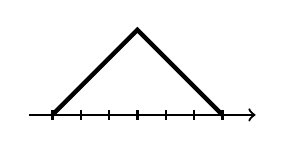
\begin{tikzpicture}[scale=.6,thick]
		\draw[->] (-.5,0)--++(4.8,0);
		\foreach \ii in {0,...,6}
		{
			\draw (\ii*.6,.1)--++(0,-.2);
		}
		\draw[ultra thick] 
		(0,0)--++(.6,.6)--++(.6,.6)
		--++(.6,.6)--++(.6,-.6)--++(.6,-.6)
		--++(.6,-.6);
	\end{tikzpicture}
	\caption{All five Dyck paths of length $2n=6$.
	The first two paths first return to zero at time $2j=2$, the 
	third path first returns to zero at time $2j=4$,
	and the last two paths first return to zero at time $2j=6$.}
	\label{fig:Dyck3}
\end{figure}

\begin{exercise}\label{exec:Dyck_Catalan}
	The number of Dyck paths of length $2n$ is equal to the Catalan number $C_n$.
\end{exercise}
\begin{proof}[Idea]
	Use the \emph{reflection principle} --- a tool used in 
	the study of random walks and Brownian motion. 
	See \url{https://en.wikipedia.org/wiki/Catalan_number#Second_proof} for details.

	Another way to count the Dyck paths is to first establish the recurrence \eqref{Catalan_recurrence}, and then use generating
	functions to solve the recurrence (see Remark \ref{rmk:from_recurrence_to_explicit_formula} below).
\end{proof}

% subsubsection dyck_paths (end)

\subsubsection{Recurrence} % (fold)
\label{ssub:recurrence}

\begin{lemma}\label{lemma:Dyck_and_recurrence}
The Catalan numbers satisfy the recurrence relation
\begin{align}\label{Catalan_recurrence}
	C_0=1,\qquad
	C_{n}=\sum_{j=0}^n C_{j-1}C_{n-j}.
\end{align}
\end{lemma}
\begin{proof}
	The easiest way to see this is by counting the Dyck paths: let the first time a Dyck path 
	reaches $0$ be $2j$, then $j$ can be any number from $1$ to $n$ (see Fig.~\ref{fig:Dyck3}). 
	The part of the Dyck path after time $2j$ is independent from the 
	part before $2j$. The number of paths 
	from $2j$ to $2n$ is exactly $C_{n-j}$. The 
	number of paths from $0$ to $2j$ 
	(with the condition that they do not get to $0$ in the meantime)
	can be seen to be $C_{j-1}$ by cutting out the first up and the 
	last down steps. This implies the recurrence.
\end{proof}

\begin{remark}\label{rmk:from_recurrence_to_explicit_formula}
	The recurrence \eqref{Catalan_recurrence} provides a way to 
	get the explicit formula \eqref{Catalan_def}. Namely, considering
	the generating function $G(z)=\sum_{n=0}^{\infty}C_n z^{n}$, 
	we see that \eqref{Catalan_recurrence} implies
	\begin{align*}
		G(z)=zG(z)^{2}+1.
	\end{align*}
	This equation on $G(z)$ has two solutions $\frac{1\pm\sqrt{1-4z}}{2z}$, 
	of which we should pick 
	$\frac{1-\sqrt{1-4z}}{2z}$ because the other solution diverges as $z\to0$.
	The Taylor expansion of this function
	is
	\begin{align*}
		\frac{1-\sqrt{1-4z}}{2z}=
		\sum_{n=0}^{\infty}\frac{1}{n+1}\binom{2n}n z^{n}=
		1+z+2 z^2+5 z^3+14 z^4+42 z^5+132 z^6+\ldots,
	\end{align*}
	which converges for $|z|<\frac14$.
	This shows that the Dyck paths are enumerated by the Catalan numbers.
\end{remark}

% subsubsection recurrence (end)

\subsubsection{Trees} % (fold)
\label{ssub:rooted_labeled_trees}

As was mentioned before, the Catalan numbers enumerate
numerous families of combinatorial objects. We will need one more family of 
such objects --- \emph{rooted ordered trees}. An ordered tree is a rooted tree (i.e., a tree with a distinguished
vertex $R$ called the \emph{root})
in which children of every vertex are linearly ordered. 
On pictures this ordering will be represented from left to right (see Fig.~\ref{fig:ordered_tree}).

\begin{figure}[htbp]
	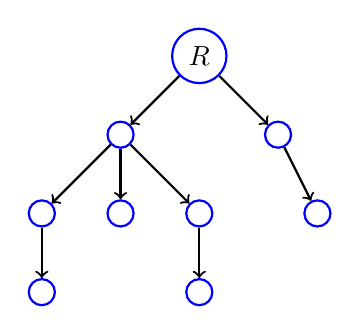
\begin{tikzpicture}[scale=1,thick,
	block/.style ={circle, draw=blue, thick ,align=center, minimum height=0.3em}]
		\node[block] (root) at (0,0) {$R$};
		\node[block] (a1) at (-1,-1) {};
		\node[block] (a2) at (1,-1) {};
		\node[block] (c1) at (1.5,-2) {};
		\node[block] (b1) at (-1,-2) {};
		\node[block] (b2) at (-2,-2) {};
		\node[block] (b3) at (0,-2) {};
		\node[block] (d1) at (0,-3) {};
		\node[block] (d2) at (-2,-3) {};
		\draw[->] (root)--(a1);
		\draw[->] (root)--(a2);
		\draw[->] (a1)--(b1);
		\draw[->] (a1)--(b2);
		\draw[->] (a1)--(b3);
		\draw[->] (a2)--(c1);
		\draw[->] (b3)--(d1);
		\draw[->] (b2)--(d2);
	\end{tikzpicture}
	\hspace{60pt}
	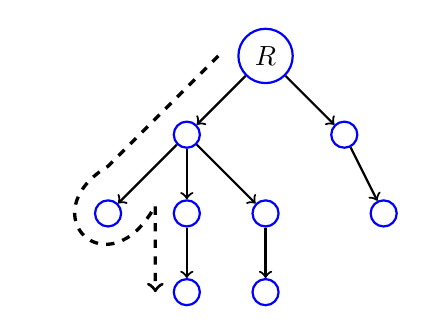
\begin{tikzpicture}[scale=1,thick,
	block/.style ={circle, draw=blue, thick ,align=center, minimum height=0.3em}]
		\node[block] (root) at (0,0) {$R$};
		\node[block] (a1) at (-1,-1) {};
		\node[block] (a2) at (1,-1) {};
		\node[block] (c1) at (1.5,-2) {};
		\node[block] (b1) at (-1,-2) {};
		\node[block] (b2) at (-2,-2) {};
		\node[block] (b3) at (0,-2) {};
		\node[block] (d1) at (0,-3) {};
		\node[block] (d2) at (-1,-3) {};
		\draw[->] (root)--(a1);
		\draw[->] (root)--(a2);
		\draw[->] (a1)--(b1);
		\draw[->] (a1)--(b2);
		\draw[->] (a1)--(b3);
		\draw[->] (a2)--(c1);
		\draw[->] (b3)--(d1);
		\draw[->] (b1)--(d2);
		\draw[->,dashed, very thick] (-.6,0)--++(-1.4,-1.4) .. controls (-3,-2) and (-2,-3) .. (-1.4,-1.9) --++ (0,-1.1);
	\end{tikzpicture}
	\caption{These trees are isomorphic as rooted trees, but are different
	as rooted ordered trees. A beginning of the walk of Exercise
	\ref{exec:trees_are_Catalan} is displayed for the second tree.}
	\label{fig:ordered_tree}
\end{figure}

\begin{figure}[htbp]
	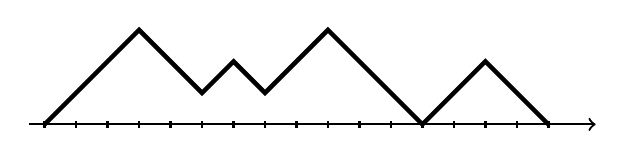
\begin{tikzpicture}[scale=.4,thick]
		\draw[->] (-.5,0)--++(18,0);
		\foreach \ii in {0,...,16}
		{
			\draw (\ii,.1)--++(0,-.2);
		}
		\draw[ultra thick] (0,0)--++(1,1)--++(1,1)--++(1,1)
		--++(1,-1)--++(1,-1)
		--++(1,1)--++(1,-1)
		--++(1,1)--++(1,1)
		--++(1,-1)--++(1,-1)--++(1,-1)
		--++(1,1)--++(1,1)
		--++(1,-1)--++(1,-1);
	\end{tikzpicture}
	\hspace{30pt}
	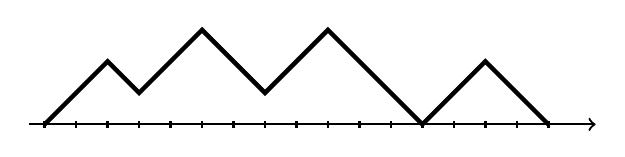
\begin{tikzpicture}[scale=.4,thick]
		\draw[->] (-.5,0)--++(18,0);
		\foreach \ii in {0,...,16}
		{
			\draw (\ii,.1)--++(0,-.2);
		}
		\draw[ultra thick] (0,0)--++(1,1)--++(1,1)--++(1,-1)
		--++(1,1)--++(1,1)
		--++(1,-1)--++(1,-1)
		--++(1,1)--++(1,1)
		--++(1,-1)--++(1,-1)--++(1,-1)
		--++(1,1)--++(1,1)
		--++(1,-1)--++(1,-1);
	\end{tikzpicture}
	\caption{Dyck paths corresponding to the rooted ordered trees on Fig.~\ref{fig:ordered_tree}
	(see Exercise \ref{exec:trees_are_Catalan}).}
	\label{fig:ordered_tree_Dyck}
\end{figure}

\begin{lemma}\label{lemma:trees_are_Catalan}
	The number of rooted ordered trees with 
	$n+1$ vertices (including the root) is equal to the Catalan number $C_n$.
\end{lemma}
\begin{proof}
	Assume that the leftmost subtree contains $j$ vertices (without the root), then the 
	rest of the tree including the root contains $n-j+1$ vertices. This readily implies the 
	recurrence \eqref{Catalan_recurrence}, which establishes the claim.
\end{proof}

\begin{exercise}\label{exec:trees_are_Catalan}
	By comparing the proof of Lemma \ref{lemma:Dyck_and_recurrence}
	and Lemma \ref{lemma:trees_are_Catalan}, come up with a bijection between
	Dyck paths and ordered rooted trees.
\end{exercise}
\begin{proof}[Idea]
	Consider the walk around the tree (such that the tree is always to the left of the walker),
	which starts to the left of the root. Let $d_k$ be the distance of the walker from the root.
	The Dyck paths corresponding to trees on Fig.~\ref{fig:ordered_tree}
	are given on Fig.~\ref{fig:ordered_tree_Dyck}.
\end{proof}

% subsubsection rooted_labeled_trees (end)

% subsection catalan_numbers (end)

\subsection{Convergence of expectations $\EE \langle x^k,L_N\rangle \to m_k$} % (fold)
\label{sub:convergence_of_expectations_}

With the Catalan preparations in place, let us return to the semicircle law. 
We would like to show that 
\begin{align}\label{desired_convergence_of_averages_in_WSCL}
	\lim_{N\to\infty}\EE \langle x^k,L_N\rangle = m_k=\begin{cases}
		0,&\textnormal{$k$ odd};\\
		C_{k/2},&\textnormal{$k$ even}.
	\end{cases}
\end{align}

First, observe that the left-hand side has the form
\begin{equation*}
\begin{split}
\EE\langle x^k,L_N\rangle&=\EE\int_{\mathbb R}x^k\,L_N(dx)\\
&=\EE\int_{\mathbb R}x^k\frac{1}{N}\sum_{i=1}^N \delta_{N^{-1/2}\lambda_i}(dx)\\
&=\EE\frac{1}{N}\sum_{i=1}^N\int_{\mathbb R}x^k\delta_{N^{-1/2}\lambda_i}(dx)\\
&=\EE\frac{1}{N}\sum_{i=1}^N (N^{-1/2}\lambda_i)^k\\
&= N^{-1-k/2}\EE \sum_{i=1}^N \lambda_i^k.
\end{split}
\end{equation*}
Since $A$ is diagonalizable (as an $N\times N$ real symmetric matrix), we have $\sum_{i=1}^N \lambda_i^k=\mathop{\mathrm{tr}}(A^k)$. We may express the trace of the $k$th power of a matrix by a $k$-fold sum of cyclic products 
\begin{align*}
	\mathop{\mathrm{tr}}(A^k)=\sum_{i_1,i_2,\ldots, i_k=1}^N a_{i_1i_2}a_{i_2i_3}\cdots a_{i_{k-1}i_k}a_{i_ki_1}.
\end{align*}
So we have
\begin{equation}\label{WSCL_proof_0}
	\EE\langle x^k,L_N\rangle
	=N^{-1-k/2} \sum_{i_1,i_2,\ldots, i_k=1}^N \EE (a_{i_1i_2}a_{i_2i_3}\cdots a_{i_{k-1}i_k}a_{i_ki_1}).
\end{equation}
Our goal now is to understand the combinatorial structure of the above big sum.
\begin{definition}
Each term of the sum can be encoded by a \emph{closed word}
$i_1\ldots i_ki_1$ of length $k+1$ (``closed'' in the sense that the word
starts and ends with the same letter). 
For example, 123241 is a closed word of length 6.
The \emph{support} of a closed word is the set of all letters participating in this word.
The support of 123241 is $\{1,2,3,4\}$.
\end{definition}

To each closed word $w$ we associate an undirected graph $G_w$ with vertices
labeled by the support of the word, edges $(i_1,i_2), (i_2,i_3),\ldots,(i_{k},i_{1})$ connecting each consecutive pair
of letters in the word. For example, if $w=123241$, then $G_w$ has four
vertices $\{1,2,3,4\}$ and five edges $\{(1,2),(2,3),(3,2),(2,4),(4,1)\}$ (see Fig.~\ref{fig:Feynman_diag_ex}).
Notice each graph $G_w$ is connected. These (and similar) graphs are sometimes referred to as Feynman diagrams.

\begin{figure}[htbp]
	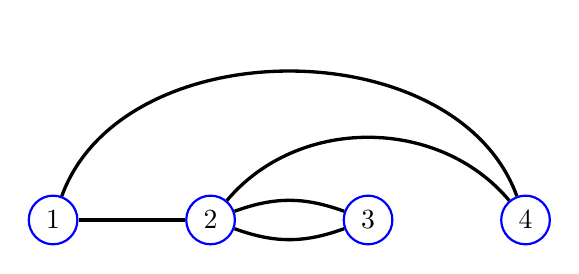
\begin{tikzpicture}[scale=2,very thick,block/.style ={circle, draw=blue, thick ,align=center, minimum height=0.3em}]
		\node[block] (n1) at (0,0) {1};
		\node[block] (n2) at (1,0) {2};
		\node[block] (n3) at (2,0) {3};
		\node[block] (n4) at (3,0) {4};
		\draw (n1)--(n2);
		\draw (n2) [out=20,in=160] to (n3);
		\draw (n2) [out=-20,in=-160] to (n3);
		\draw (n2) [out=50,in=130] to (n4);
		\draw (n4) [out=110,in=70] to (n1);
	\end{tikzpicture}
	\caption{Graph $G_w$ corresponding to the word $w=123241$.}
	\label{fig:Feynman_diag_ex}
\end{figure}

Let $N_{i_1i_2}^w$ be the number of distinct edges connecting $i_1$ to $i_2$ in $G_w$. In our running example we have $N_{12}^w=1$ and $N_{23}^w=2$.
Each edge may be a \emph{self} edge such as $(1,1)$, or it can be an edge \emph{connecting} distinct vertices such as $(2,3)$.

With this notation we have
\begin{equation}\label{WSCL_proof_1}
	\EE a_{i_1i_2}a_{i_2i_3}\cdots a_{i_{k-1}i_k}a_{i_ki_1}=
	\prod_{\substack{\textnormal{self $e$}\\e\in G_{i_1\cdots i_ki_1}}}\EE a_{11}^{N_e}
	\prod_{\substack{\textnormal{connecting $e$}\\ e\in G_{i_1\cdots i_ki_1}}}\EE a_{12}^{N_e},
\end{equation}
since all diagonal elements are iid, and all the elements above the diagonal are iid.
Here the product runs over all possible distinct edges in the graph of the word.

In order for the expectation
\eqref{WSCL_proof_1} to be nonzero, we must have the following properties:
\begin{itemize}
	\item
	Since $\EE a_{ij}=0$, each edge in $G_{i_1\cdots i_ki_1}$ must have 
	$N_e\ge2$..
	\item The graph $G_{i_1\cdots i_ki_1}$ has $k+1$ edges, and so it can have
	at most $1+k/2$ vertices.
\end{itemize}

Now let us look at the sum \eqref{WSCL_proof_0} as a whole. 
Call two graphs
\emph{equivalent}
if they differ only by relabeling the vertices.
Note that the 
expectations 
of the form
\eqref{WSCL_proof_1}
coming from equivalent graphs are the same. If a graph has $t$ vertices, then there are 
$N^{\downarrow t}:=N(N-1)\ldots(N-t+1)$ ways to relabel the vertices 
to get an equivalent graph. This implies that the sum
\eqref{WSCL_proof_0} can be rewritten as
\begin{align}\label{WSCL_proof_2}
	\EE\langle x^k, L_N\rangle=\sum_{t=0}^{1+\lfloor k/2\rfloor}\frac{N^{\downarrow t}}{N^{1+k/2}}
	\underbrace{\sum_{G_w\in\text{EqClass}_t}\,
	\prod_{\substack{\text{self } e\\e\in G_{w}}}\EE a_{11}^{N_e}
	\prod_{\substack{\text{connecting } e\\ e\in G_{w}}}\EE a_{12}^{N_e}}_{(*)},
\end{align}
where by $\text{EqClass}_t$ we have denoted the set of equivalence classes
of graphs $G_w$ corresponding to closed word, having $t$ vertices and $k+1$ edges, and 
also having $N_e\ge2$ for each edge.

Clearly, for fixed $t$ and $k$, the expression $(*)$ above does not depend on $N$
and is finite. Also, since $N^{\downarrow t}=O(N^{t})$, 
the sum \eqref{WSCL_proof_2} vanishes as $N\to\infty$
unless $t=1+k/2$. Because $t\le \lfloor k/2\rfloor$, this is possible only
for $k$ even. Therefore,
$\EE\langle x^k, L_N\rangle$ converges to zero if $k$ is odd.

Now consider the case when $k$ is even and $t=1+k/2$. Then the graph corresponding to each word
$i_1 \ldots i_ki_1$ has $k+1$ edges, $1+k/2$ vertices, 
and $N_e\ge2$ for each edge. Hence, gluing together pairs of edges connecting 
the same vertices, we see that the graph 
$G_{i_1 \ldots i_ki_1}$ must be a \emph{tree} (see Fig.~\ref{fig:Wigner_word}).\footnote{The words which correspond to
such trees 
contributing to \eqref{WSCL_proof_2}
are sometimes referred to as \emph{Wigner words}.}
In particular, there are no self edges and $N_e=2$ for each connecting edge. This implies that 
\begin{align*}
	\lim_{N\to\infty}\EE\langle x^k, L_N\rangle=\big|\text{EqClass}_{1+k/2}\big|.
\end{align*}

\begin{figure}[htbp]
	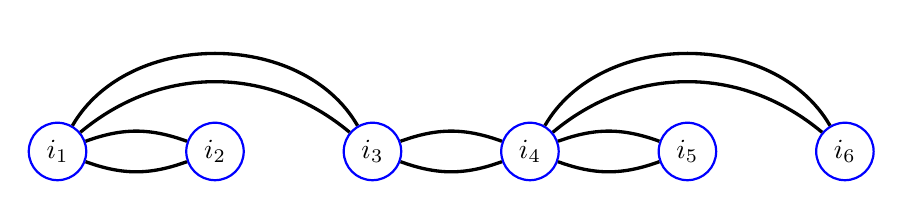
\begin{tikzpicture}[scale=2,very thick,block/.style ={circle, draw=blue, thick ,align=center, minimum height=0.3em}]
		\node[block] (n1) at (0,0) {$i_1$};
		\node[block] (n2) at (1,0) {$i_2$};
		\node[block] (n3) at (2,0) {$i_3$};
		\node[block] (n4) at (3,0) {$i_4$};
		\node[block] (n5) at (4,0) {$i_5$};
		\node[block] (n6) at (5,0) {$i_6$};
		\draw (n1) [out=20,in=160] to (n2);
		\draw (n1) [out=-20,in=-160] to (n2);
		\draw (n1) [out=40,in=140] to (n3);
		\draw (n1) [out=60,in=120] to (n3);
		\draw (n3) [out=20,in=160] to (n4);
		\draw (n3) [out=-20,in=-160] to (n4);
		\draw (n4) [out=20,in=160] to (n5);
		\draw (n4) [out=-20,in=-160] to (n5);
		\draw (n4) [out=40,in=140] to (n6);
		\draw (n4) [out=60,in=120] to (n6);
	\end{tikzpicture}
	\caption{A graph $G_w$ corresponding to a Wigner word 
	$w=i_{1}i_3i_4i_5i_4i_6i_4i_3i_1i_2i_1$
	which nontrivially contributes to the expansion \eqref{WSCL_proof_2}. 
	Here $k=10$.}
	\label{fig:Wigner_word}
\end{figure}	
\begin{figure}[htbp]
	\raisebox{50pt}{\scalebox{.8}{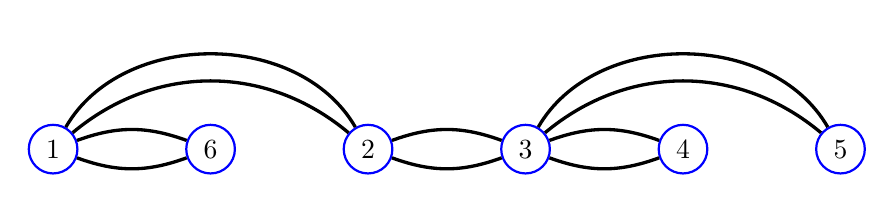
\begin{tikzpicture}[scale=2,very thick,block/.style ={circle, draw=blue, thick ,align=center, minimum height=0.3em}]
		\node[block] (n1) at (0,0) {$1$};
		\node[block] (n2) at (1,0) {$6$};
		\node[block] (n3) at (2,0) {$2$};
		\node[block] (n4) at (3,0) {$3$};
		\node[block] (n5) at (4,0) {$4$};
		\node[block] (n6) at (5,0) {$5$};
		\draw (n1) [out=20,in=160] to (n2);
		\draw (n1) [out=-20,in=-160] to (n2);
		\draw (n1) [out=40,in=140] to (n3);
		\draw (n1) [out=60,in=120] to (n3);
		\draw (n3) [out=20,in=160] to (n4);
		\draw (n3) [out=-20,in=-160] to (n4);
		\draw (n4) [out=20,in=160] to (n5);
		\draw (n4) [out=-20,in=-160] to (n5);
		\draw (n4) [out=40,in=140] to (n6);
		\draw (n4) [out=60,in=120] to (n6);
	\end{tikzpicture}}}
	\hspace{40pt}
	\scalebox{.8}{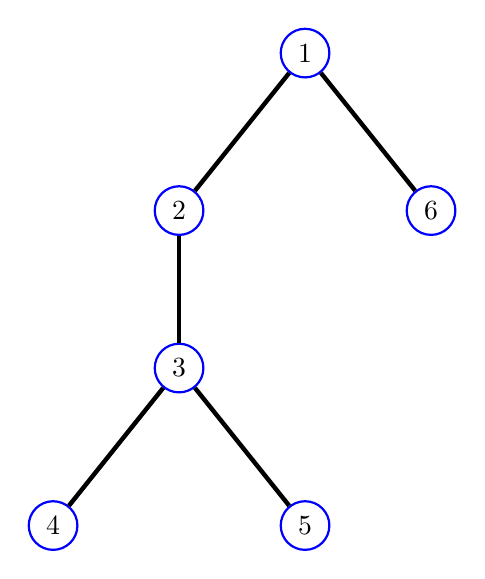
\begin{tikzpicture}[scale=2,very thick,block/.style ={circle, draw=blue, thick ,align=center, minimum height=0.3em}]
		\node[block] (n1) at (0,0) {$1$};
		\node[block] (n2) at (.8,-1) {$6$};
		\node[block] (n3) at (-.8,-1) {$2$};
		\node[block] (n4) at (-.8,-2) {$3$};
		\node[block] (n5) at (-1.6,-3) {$4$};
		\node[block] (n6) at (0,-3) {$5$};
		\draw[ultra thick] (n1)--(n3);
		\draw[ultra thick] (n1)--(n2);
		\draw[ultra thick] (n3)--(n4);
		\draw[ultra thick] (n4)--(n5);
		\draw[ultra thick] (n4)--(n6);
	\end{tikzpicture}}
	\caption{A representative graph 
	$G_w\in \text{EqClass}_{1+k/2}$ corresponding to the graph as on
	Fig.~\ref{fig:Wigner_word} (left), and its representation as a rooted ordered tree (right).}
	\label{fig:Wigner_word_representative}
\end{figure}

To count the number of trees $G_w\in\text{EqClass}_{1+k/2}$, 
let us choose representatives $w=v_1 \ldots v_{k+1}$,
such that for each $i=1,\ldots,k+1$, the set $\{1,2,\ldots,v_i\}$
is an interval in $\{1,2,\ldots,N\}$ beginning at $1$
(thus, $v_1=v_{k+1}=1$).
\begin{exercise}
	There is a unique way of choosing such representatives.
\end{exercise}
Let the vertex $1$ be the root $R$, and clearly the order coming from the word
defines an order on this rooted tree (see Fig.~\ref{fig:Wigner_word_representative}). This implies that 
$\big|\text{EqClass}_{1+k/2}\big|=C_k$, and
finally proves the desired convergence \eqref{desired_convergence_of_averages_in_WSCL}.

% subsection convergence_of_expectations_ (end)

\lect{1/27/2016}

\subsection{An example of counting terms in the expansion (\ref{WSCL_proof_0})} % (fold)
\label{sub:an_example_WSCL_proof}

Before proceeding to finish the proof, let us consider one example 
how expansion \eqref{WSCL_proof_0} works 
for $k=6$.

\begin{exercise}
How go get $ C_3 = 5 $ when calculating $ \EE(\mathop{\mathrm{tr}}( A^6 ) )$.
\end{exercise}
\begin{proof}[Solution]
	We want to show how

	\begin{equation*}
	\EE( \, \text{Tr}( A^6 ) \, ) = N^{ -1 - 3 } \sum_{ i_1 , \ldots, i_6 = 1 }^N \EE \left( a_{ i_1, i_2 } \cdot a_{ i_2, i_3 } \cdots a_{ i_5, i_6 } \cdot a_{ i_6, i_1 } \right) \xrightarrow[ N \to \infty ]{} 5.
	\end{equation*}

	We need to determine which terms are non-zero and how many such terms there are.  If there are 5 or 6 independent indices, we get a product of expected values of independent random variables with expected value zero, so these terms do not contribute.  If there are 3 or fewer independent indices, there are not enough terms to overcome the factor of $ N^{ -4 } $, so these terms do not contribute in the limit.  Thus we are interested in non-zero terms with 4 independent indices.
	One can check that there are 5 types of such terms:

	\begin{enumerate}

	\item
	\begin{equation*}
	\underbrace{ ( i_1, i_2 ) , ( i_2 , i_1 ) }, \quad \underbrace{ ( i_1, i_3 ) , ( i_3, i_1 ) }, \quad \underbrace{ ( i_1, i_4 ), ( i_4, i_1 ) }
	\end{equation*}

	\item
	\begin{equation*}
	\underbrace{ ( i_1, i_2 ) , \quad \underbrace{ ( i_2 , i_3 ) , ( i_3, i_2 ) } , \quad ( i_2, i_1 ) } , \quad \underbrace{ ( i_1, i_4 ), ( i_4, i_1 ) }
	\end{equation*}

	\item
	\begin{equation*}
	\underbrace{ ( i_1, i_2 ) , \quad \underbrace{ ( i_2 , i_3 ) , ( i_3, i_2 ) } , \quad \underbrace{ ( i_2, i_4 ) , ( i_4, i_2 ) }, \quad ( i_2, i_1 ) } 
	\end{equation*}

	\item
	\begin{equation*}
	\underbrace{ ( i_1, i_2 ) , \quad \underbrace{ ( i_2 , i_3 ) , \quad \underbrace{ ( i_3, i_4 ) , ( i_4, i_3 ) }, \quad ( i_3, i_2 ) } , \quad ( i_2, i_1 ) } 
	\end{equation*}

	\item
	\begin{equation*}
	\underbrace{ ( i_1, i_2 ) , ( i_2 , i_1 ) } , \quad \underbrace{ ( i_1, i_3 ) , \quad \underbrace{ ( i_3, i_4 ) , ( i_4, i_3 ) } , \quad ( i_3, i_1 ) }
	\end{equation*}

	\end{enumerate}

	These sequences bijectively correspond to non-crossing pair partitions of 6 elements.
	These partitions are in bijection with Dyck paths of length 6
	(shown on Fig.~\ref{fig:Dyck3}), and are enumerated by the Catalan number $C_3=5$.

	For each of these patterns, there are $ N ( N - 1 ) ( N - 2 ) ( N - 3 ) \sim N^4 $ terms in the sum, and each term is a product of the expected value of the squares of three independent off-diagonal random variables with expected value 0 and variance 1, like
	\begin{align*}
	\EE ( a_{ i_1, i_2 } \cdot a_{ i_2 , i_1 } \cdot a_{ i_1, i_3 } \cdot a_{ i_3, i_1 } \cdot a_{ i_1, i_4 } \cdot a_{ i_4, i_1 } ) &= \EE( a_{ i_1, i_2 }^2 ) \cdot \EE( a_{ i_1, i_3 }^2 ) \cdot \EE( a_{ i_1, i_4 }^2 ) = 1.
	\end{align*}
	So in the limit we get the Catalan number $ C_3 = 5 $.
\end{proof}

% subsection an_example (end)

\subsection{Variances of $\langle x^k,L_N\rangle$} % (fold)
\label{sub:variances_langle_x_k_l_nrangleto0_}

Let us now show that the variances vanish in the limit:
\begin{equation}\label{Variance_to_zero_WSCL}
\EE ( \, \langle x^k , L_N \rangle^2 ) - \left( \, \EE ( \, \langle x^k , L_N \rangle \, ) \, \right)^2 \xrightarrow[ N \to \infty ]{} 0.
\end{equation}
Recall that
\begin{equation*}
\langle x^k , L_N \rangle = N^{ -1 - k/2 } \sum_{ \vec{i} = i_1 , \ldots, i_k = 1 }^n a_{ i_1, i_2 } \cdots a_{ i_k , i_1 }.
\end{equation*}
Now, writing $ a_{ \vec{i} } $ for $ a_{ i_1, i_2 } \cdots a_{ i_k , i_1 } $, we have
\begin{equation*}
\EE ( \, \langle x^k , L_N \rangle^2 ) - \left( \, \EE ( \, \langle x^k , L_N \rangle \, ) \, \right)^2 = N^{ -2 - k } \sum_{ \vec{i} , \vec{j} } \left(  \EE \left( a_{ \vec{i} } \cdot a_{ \vec{j} } \right) - \EE ( a_{ \vec{i} } ) \cdot \EE ( a_{ \vec{j} } ) \, \right).
\end{equation*}
If the graphs $ G_{ \vec{i} } $ and $ G_{ \vec{j} } $ 
(corresponding to the words $i_1 \ldots i_ki_1$ and $j_1 \ldots j_kj_1$,
respectively)
do not share common edges, 
then the corresponding random variables $ a_{ \vec{i} } $ and $ a_{ \vec{j} } $ 
are independent, and so $ \EE( a_{ \vec{ i } } \cdot a_{ \vec{j} } ) = \EE ( a_{ \vec{i} } ) \cdot \EE( a_{ \vec{j} } ) $.  
Thus we are only interested in the terms for which edges of the 
graphs $ G_{ \vec{i} } $ and $ G_{ \vec{j} } $ overlap.

\begin{example}\label{ex:GiGj_variance_in_WSCL}
	For instance, if $ \vec{i} = ( 1, 2, 3, 2 , 1 ) $ and $ \vec{j} = ( 1, 2, 1, 1, 1 ) $, then
	\begin{align*}
	\EE( a_{ \vec{i} } ) = \EE( a_{ i_1, i_2 } \cdot a_{ i_2, i_3 } \cdot a_{ i_3, i_2 } \cdot a_{ i_2, i_1 } ) &= \EE( a_{ 1, 2 }^2 )^2 = 1;
	\\\EE( a_{ \vec{j} } ) = \EE( a_{ i_1, i_2 } \cdot a_{ i_2, i_1 } \cdot a_{ i_1, i_1 } \cdot a_{ i_1, i_1 } ) &= \EE( a_{ 1, 2 }^2 ) \cdot \EE( a_{ 1,1 } ) = 2;
	\\\EE( a_{ i_1, i_2 } \cdot a_{ i_2, i_3 } \cdot a_{ i_3, i_2 } \cdot a_{ i_2, i_1 } \cdot a_{ i_1, i_2 } \cdot a_{ i_2, i_1 } \cdot a_{ i_1, i_1 } \cdot a_{ i_1, i_1 } ) &= \EE( a_{ i_1, i_2 }^4 ) \cdot \EE( a_{ i_2, i_3 }^2 ) \cdot \EE( a_{ i_1, i_1 }^2 ) = 2 \EE( a_{ 1, 2 }^4 ).
	\end{align*}
	The corresponding graphs are given on Fig.~\ref{fig:GiGj_variance_in_WSCL}.
\end{example}
\begin{figure}[htbp]
	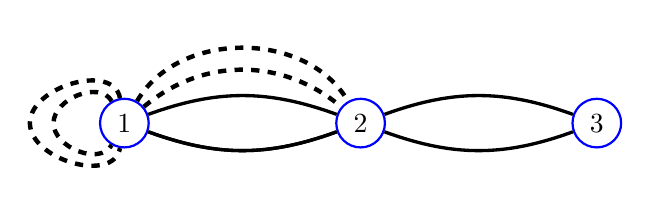
\begin{tikzpicture}[scale=3,very thick,block/.style ={circle, draw=blue, thick ,align=center, minimum height=0.3em}]
		\node[block] (n1) at (0,0) {$1$};
		\node[block] (n2) at (1,0) {$2$};
		\node[block] (n3) at (2,0) {$3$};
		\draw (n1) [out=20,in=160] to (n2);
		\draw (n1) [out=-20,in=-160] to (n2);
		\draw[dashed, ultra thick] (n1) [out=40,in=140] to (n2);
		\draw[dashed, ultra thick] (n1) [out=60,in=120] to (n2);
		\draw[dashed, ultra thick] (n1) [out=120,in=90] to (-.3,0) [out=-90,in=-120] to (n1);
		\draw[dashed, ultra thick] (n1) [out=100,in=90] to (-.4,0) [out=-90,in=-100] to (n1);
		\draw (n1) [out=-20,in=-160] to (n2);
		\draw (n2) [out=20,in=160] to (n3);
		\draw (n2) [out=-20,in=-160] to (n3);
	\end{tikzpicture}
	\caption{Graphs $ G_{ \vec{i} } $ (solid lines) and $ G_{ \vec{j} } $ (dashed lines) in Example \ref{ex:GiGj_variance_in_WSCL}.}
	\label{fig:GiGj_variance_in_WSCL}
\end{figure}

We now argue similarly to the proof given in \S \ref{sub:convergence_of_expectations_}
(for the convergence of the first moments). Namely, 
in order for $ \EE ( a_{ \vec{i} } \cdot a_{ \vec{j} } ) - \EE( a_{ \vec{i} } ) \EE( a_{ \vec{j} } ) $ to be non-zero 
we must have the following:
\begin{itemize}
	\item Since
	$ \EE( a_{ i j } ) = 0$,
	the graphs need to have $ N_e \ge 2 $;
	\item The graphs $ G_{ \vec{i} } $ and $ G_{ \vec{j} } $ need to share some edges.
\end{itemize}

If the combined graph has $ t $ vertices, there are $ N^{ \downarrow t } = N ( N - 1 ) \cdots ( N - t + 1 ) $ equivalent classes of graphs.  Thus, the variance takes the form
\begin{equation*}
\EE ( \, \langle x^k , L_N \rangle^2 ) - \left( \, \EE ( \, \langle x^k , L_N \rangle \, ) \, \right)^2 = N^{ -2 - k } \sum_{ t = 1 }^{ 2k } N^{ \downarrow t } \underbrace{ \left[ \sum_{ \substack{ \text{equiv. classes} \\ \text{ of graphs with} \\ \text{ $2k$ vertices } } } ( \text{finite products of finite moments} )\right] }_{ \text{ finite and independent of $N$ } }
\end{equation*}
Thus, we must have $ t \ge k + 2 $ in order to have a nonzero contribution as $ N \to \infty $.  
The associated graphs have $ N_e \ge 2 $ and are connected (since $ G_{ \vec{i} } $ and $ G_{ \vec{j} } $ are connected and overlap).
There are totally $ 2 k $ edges with multiplicities, thus  $\le k $ double edges.
We conclude that there are no such graphs, and so there are no nonzero contributions to the 
variance in the limit as $N\to\infty$. This 
completes the proof of \eqref{Variance_to_zero_WSCL}.

\begin{remark}
	Remark: by a similar argument, $ t = k + 1 $ also cannot contribute.
	Indeed, the combined graph of $ G_{ \vec{i} } $ and $ G_{ \vec{j} } $
	has $\le k$ double edges and $k+1$ vertices so it must be a tree
	(in the same sense of gluing edges as in \S \ref{sub:convergence_of_expectations_} above).
	However, as $ G_{ \vec{i} } $ and $ G_{ \vec{j} } $ must also overlap (i.e., share common edges),
	there are no such trees.
	This implies a better estimate on the variance:
	\begin{equation*}
	\EE \left( \, \langle x^k , L_N \rangle^2 \, \right) - \EE \left( \, \langle x^k , L_N \rangle \, \right)^2 = O( N^{-2} ) ,
	\qquad
	N\to\infty.
	\end{equation*}
	This estimate can in fact be used to show almost-sure convergence to the semi-circular law.
\end{remark}

% subsection variances_langle_x_k_l_nrangleto0_ (end)

\subsection{Estimates and completing the proof} % (fold)
\label{sub:completing_the_proof_WSCL}

% subsection completing_the_proof (end)

\subsection{Related laws of large numbers for random matrix spectra} % (fold)
\label{sub:remarks_on_the_semicircle_law_for_real_wigner_matrices}

Let us mention two relatives of the Wigner semicircle law which can be proven by similar 
methods of moments and
trees counting.

\subsubsection{Complex Wigner matrices} % (fold)
\label{ssub:complex_wigner_matrices}
	
The first is the law of large numbers for complex (Hermitian) random Wigner
matrices $A= ( a_{ i j } )_{i,j=1}^{N}$, in which
\begin{itemize}
	\item $ \overline{ a_{ i j } } = a_{ j i } $, $i\le j$,
	are complex-valued independent random variables.
	\item The diagonal elements
	$ a_{ i i } $ are iid real valued with mean $0$ and variance $2$.
	\item $ a_{ i j } $ with $ i < j $ are iid complex random variables
	with expected value 0 and (complex) variance 1.
	On other words, $a_{ij}=x_{ij}+y_{ij}$, where $x_{ij}$ and $y_{ij}$ are independent
	real random variables with mean $0$ and variance $\frac12$. This implies that 
	$\EE a_{ij}^{2}=0$ and $\EE |a_{ij}|^{2}=1$.
	\item All moments $\EE|a_{ij}|^{k}$ are finite.
\end{itemize}
Defining $L_N$ in in the same way by \eqref{EmpiricalDistributionOfEigenvalues}
(note that the eigenvalues of $A$ are real because it is Hermitian),
we still have the semicircle law: 
$ L_N \rightarrow \SC $ weakly in probability.

There also exist laws of large numbers
for complex eigenvalues of random matrices,
and typical is the \emph{circular law} stating
that the eigenvalues of a random matrix with iid 
entries are distributed uniformly inside a unit disc on the 
complex plane (cf. Remark \ref{rmk:complex_eigenvalues}).


% subsubsection complex_wigner_matrices (end)

\subsubsection{Marchenko--Pastur law} % (fold)
\label{ssub:marchenko_pastur_law}

The second is the Marchenko--Pastur law \cite{MarchenkoPastur}
for Wishart matrices (random sample covariance matrices). The Wishart ensemble is defined as follows.
Let $ Y $ be an $ N \times M $ matrix of iid real-valued random variables with mean 0 and variance 1. 
Then, by definition, $ W = Y Y^\text{T} $ is called a \emph{Wishart} $ N \times N $ random matrix.
It is a symmetric random matrix which is, moreover, positive definite.
Therefore, all its eigenvalues are real and nonnegative.
\begin{remark}
	If the entries of $ Y $ are Gaussian, then the entries of $ W $ are sums of squares of Gaussians, 
	so they have chi square distributions --- a type of distribution
	arising when studying sample covariance matrices of Gaussian random vectors.
\end{remark}

Suppose $ M / N \to \alpha \in [ 1, \infty ) $. The Marchenko--Pastur law states that
\begin{equation*}
L_N = \frac{ 1 }{ N } \sum_{ i = 1 }^N \delta_{ \lambda_i / \sqrt{N} } \to S_\alpha 
\end{equation*}
weakly in probability. Here
$ S_\alpha $, $\alpha\in[1,\infty)$ are the Marchenko--Pastur distributions defined as follows.
Set
\begin{equation*}
b_\pm = ( 1 \pm \sqrt{\alpha} )^2.
\end{equation*}
Then the density function of $ S_\alpha $ is
\begin{equation*}
f_\alpha( x ) = \frac{ \sqrt{ ( x - b_- ) ( b_+ - x ) } }{ 2 \pi x }, \qquad b_- \le x \le b_+
\end{equation*}
which looks as on Fig.~\ref{fig:MP_law}.
\begin{figure}[htbp]
	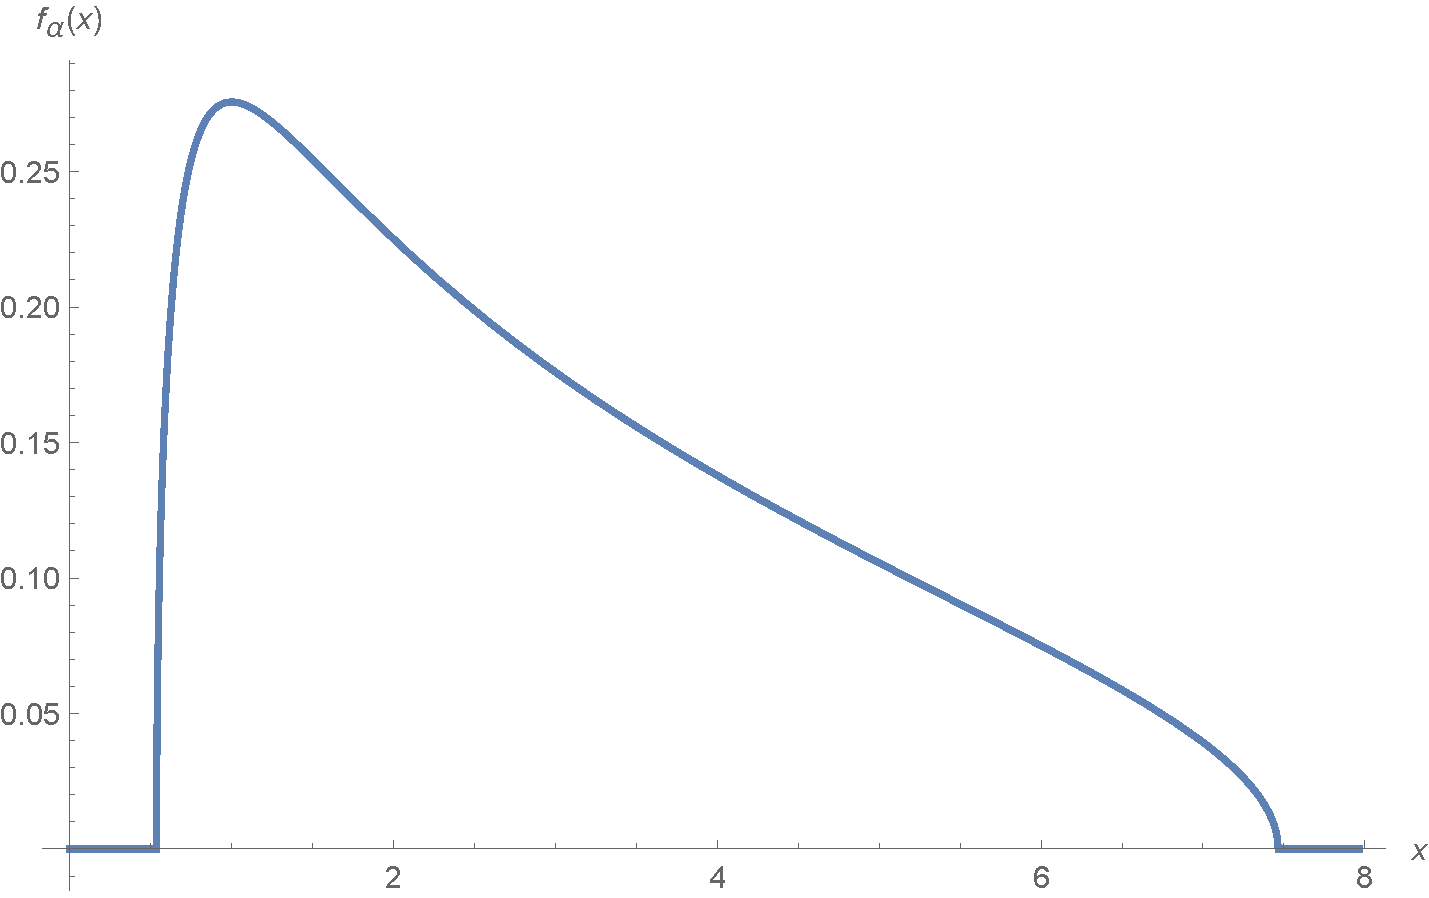
\includegraphics[width=.5\textwidth]{img/Marchenko-Pastur.pdf}
	\caption{The Marchenko--Pastur density $f_\alpha(x)$ for $\alpha=3$.}
	\label{fig:MP_law}
\end{figure}

Note that if $ M \gg N $, then the random matrices $W$ are likely to be non-degenerate, so the distribution does not hit zero.
In fact, the distribution $ S_1 $ corresponding to $\alpha=1$
is the image of the semicircle law $ \SC $ under the squaring map $ x \mapsto x^2 $.


% subsubsection marchenko_pastur_law (end)

% subsection remarks_on_the_semicircle_law_for_real_wigner_matrices (end)

% section wigner_s_semicircle_law (end)

\lect{2/1/2016}

\section{Elements of free probability} % (fold)
\label{sec:elements_of_free_probability}

% section elements_of_free_probability (end)

\lect{2/3/2016}


\bibliography{bib}
\bibliographystyle{amsalpha}

\end{document}